\section{Details on Machine Learning Methods}
\subsection{Decision Tree}
\subsubsection{Introduction}
Decision trees are a statistical learning method used both in the classification and regression setting. They are non-parametric models, meaning that they don't approximate a function $\hat{f}$ to describe the relationship between the features and target, but are classifying data by inferring a hierarchical decision structure (the decision tree) \cite{introStats}.

Decision trees are based on the idea of segmenting the feature space into a number of simple regions (rectangles in 2-dimensional space, cubes in 3-dimensional space, etc.). The challenge of tree-based learning methods is to identify the regions that best separate the classes. Mathematically, a loss function, ie. cross-entropy, gini-impurity or 0-1 loss, should be minimised for each data point in the training split, st.

$$
\text{min}\left\{\sum_{j=1}^J\sum_{i\in{R_J}} \text{loss(}y_i, \hat{y}_{R_j}\text{)}\right\}
$$
\vspace{5pt}

However, it is computationally infeasible to consider every possible partition of the feature space into $J$ regions and evaluate the loss. For this reason, a top-down, greedy approach, known as recursive binary splitting is used to construct the decision tree in a computationally light fashion.

Recursive binary splitting is a recursive algorithm that splits a given partition of the training set (node) into the two (hence the name \textit{binary} splitting) partitions that best separate the classes in the original partition. It thus finds the cut point $s$ for a feature $X_i$ that forms two sets $\{X| X_i<s\}$ and $\{X|X_i\ge s\}$ that minimise the weighted loss of both regions. 
The decision tree is then built by recursively applying this algorithm, until some stopping criterion is reached, or all regions are pure (ie. all training samples in a decision region are of a single class). The final prediction is based on identifying which region a new data point belongs to and then predicting the majority class in that region. 

\subsubsection{Decision Tree Model Selection}
%Having implemented the \class{DecisionTreeClassifier()}, the challenge arises of which set of hyper parameters in the training phase produces a classifier, that best generalises to unseen data. Particularly, we wish to find the classifier that is neither oversimplifying (high bias, low variance model) nor overfitting (low bias, high variance model). 

% To find the configuration of hyper parameters that best generalise, we used \class{GridSearchCV} from \textit{sci-kit learn}. It allows to search a set of hyper parameter configurations for the best-generalising performance using 5-fold cross validation by choosing the model that achieves best average validation performance on some scoring-criterion. 

The final decision tree classifier is a pipeline of a \code{StandardScaler} instance, that was fitted on the training split and a \code{DecisionTreeClassifier} instance. For the scope of this project a combination of the hyper parameters \code{criterion}, \code{splitter}, \code{max_features} and \code{max_depth} of the tree were checked within a grid search.
\newline

\begin{comment}
\begin{lstlisting}[language=Python, caption=DecisionTreeClassifier Pipeline and GridSearch Setup, label=dt_pipeline]
    # model pipeline 
    pipe = Pipeline(steps=[('scaler', scaler),
                           ('decision_tree', DecisionTreeClassifier(random_state=1))])

    # define hyper parameters to grid search
    params = {
            'decision_tree__criterion': ['gini', 'entropy'],
            'decision_tree__max_depth': list(range(1, 10)),
            'decision_tree__max_features': list(range(1, 10)),
            'decision_tree__splitter': ['best', 'random'] 
            }
\end{lstlisting}
\end{comment}

The grid search ran over all possible combinations of hyper parameters defined. For each setting it fitted five models on four (randomised) folds and validated the performance of the model on the remaining split. It then computed the averaged accuracy score on the validation splits that occurred within the training and returned the model configuration that maximised the performance of the model on the validation splits. The best generalising decision tree was found to use \textit{entropy-impurity} as a loss-function, is trained to maximum depth of five and considers eight features for each split. 

\subsubsection{Decision Tree Performance Evaluation}
The best generalising model achieved an averaged accuracy score in the cross-validation splits of 70\%, which is the estimated performance on unseen data. Because of that, it is surprising to see a test accuracy of only 62\%. The variation in the two metrics is likely occurs, because both the training and test split are rather small, making it prone to random variation. From the classification report it becomes clear that the decision tree struggles with separating classes 1, 2 and 3 from each other. In contrast, the model does rather well on the more separated classes 6 and 7 with an F1-Score of 80\% each.  
\newline

\begin{table}[!ht]
\begin{subtable}[c]{0.4\textwidth}
\footnotesize
\centering
\begin{tabular}{ c | c }
 \toprule
 Evaluation Metric & Score  \\
 \midrule 
 Training Accuracy & 87\% \\
 Validation Accuracy (during CV) & 70\% \\
 Test Accuracy & 62\% \\
 \bottomrule
\end{tabular}
\captionsetup{justification=centering,margin=1cm}
\subcaption{Decision Tree Accuracy Scores on Training, Validation and Test Split}
\end{subtable}
\begin{subtable}[c]{0.6\textwidth}
\footnotesize
\centering
\begin{tabular}{c | c c c r}
Class & Precision & Recall & F-Score & Support\\
\midrule
1   &    0.68  &    0.62  &    0.65  &  21 \\
2   &    0.64  &    0.61  &    0.62  &  23 \\
3   &    0.25  &    0.20  &    0.22  &   5 \\
5   &    0.33  &    1.00  &    0.50  &   4 \\
6   &    1.00  &    0.67  &    0.80  &   3 \\
7   &    1.00  &    0.67  &    0.80  &   9 \\
\midrule
    accuracy   &           &         &    0.62   &   65 \\
   macro avg   &    0.65   &   0.63  &    0.60   &   65 \\
weighted avg   &    0.67   &   0.62  &    0.63   &   65 \\
\end{tabular}
\captionsetup{justification=centering,margin=1cm}
\subcaption{Decision Tree Classification Report on Test Split}
\end{subtable}
\caption{Decision Tree Performance Evaluation}
\label{dt_evaluation}
\end{table}


\subsubsection{Visualization of Decision Tree}
Figure \ref{dt_visualisation} shows a visualisation of the constructed decision tree. At each level of the tree the node carries information about the decision rule applied at the specific node, the loss-value (ie. gini impurity), the number of samples considered and the majority class in the node. 

One interesting observation is that the feature \textit{barium} is used at depth 2 to separate a pure leaf with class 7 (headlamp) off. This was expected from inspecting the feature distribution in each class in Section 3, since the feature distribution of class 7 was distinct for the feature \textit{batrium}. 

\begin{figure}[ht]
\centering
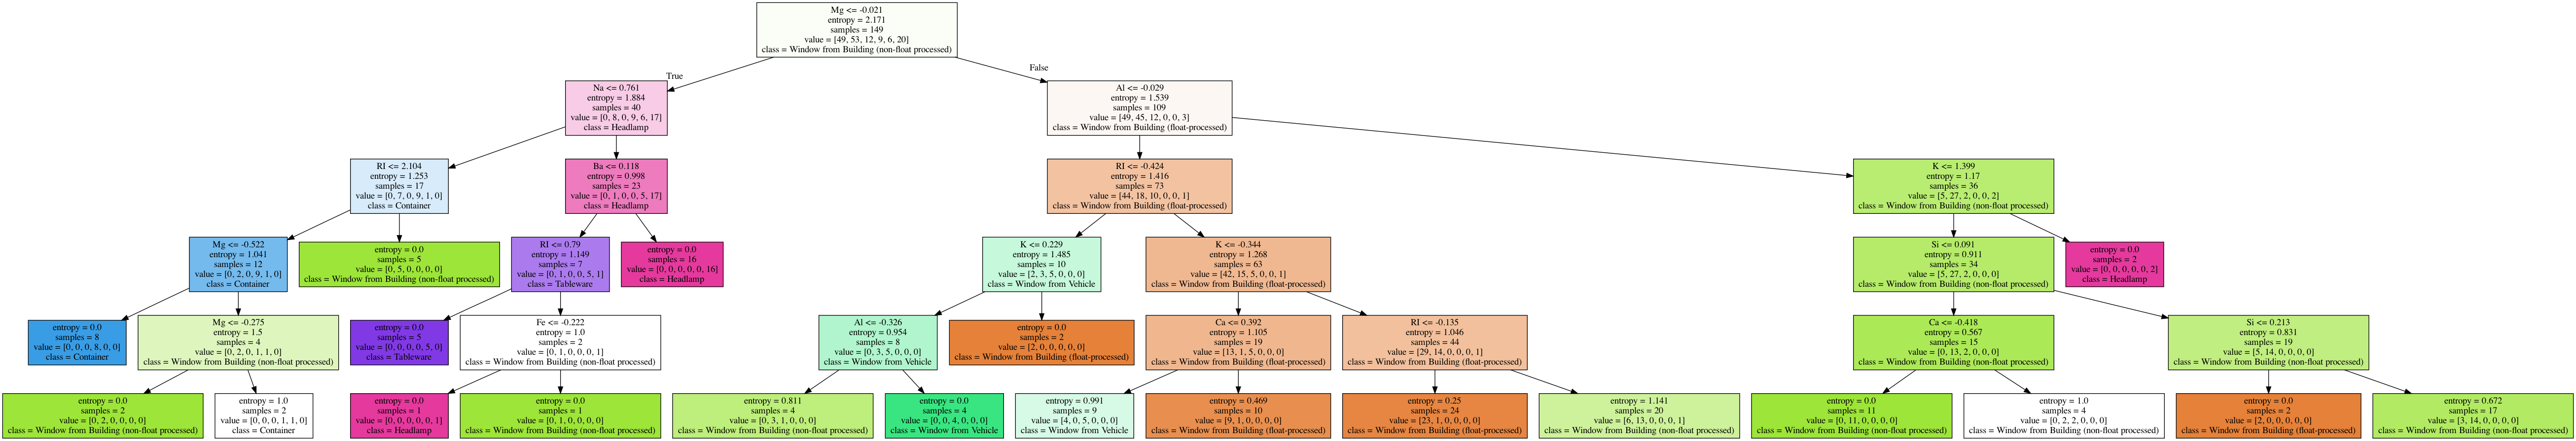
\includegraphics[scale=0.09]{figures/graphviz_sklearn_dt.png}
\caption{Visualised Decision Tree}
\label{dt_visualisation}
\end{figure}


\subsection{Neural Network}
\subsubsection{Introduction}
A feed-forward neural network is a machine learning algorithm that constructs
a nonlinear (decision) function $\hat{f}(X)$ that tries to approximate the true relationship between some feature matrix $X$ and a target vector $y$ \cite{introStats}. In each layer of the neural network, an activation function is applied to ensure the non-linearity of the decision function $\hat{f}$.

To train a neural network a loss function (e.g. cross entropy) is minimised using the technique of back-propagation. The algorithm computes the gradient of the loss with respect to all the weights and biases. This gradient
is then used to tweak the parameters to reduce the error using a gradient descent step. The process is repeated until the neural network converges to the desired solution \cite{handsonML}.

When dealing with a classification problem the response $y$ is a vector produced by the last layer (the output layer) with a soft-max function as its activation, ensuring that the sum of elements is one ($\sum_{i=1}^{i=k}y_i = 1$) and each respective element is in the range of 0 to 1 ($0\ge y_i \ge 1 \ \ y_i \forall y$).  
Therefore the individual scalars of the vector $y$ can be interpreted as probabilities that a data point that was fed forward through the network belongs to the different classes. The prediction is then made to the class with the largest probability. 

\subsubsection{Neural Network Model Selection}
Since the custom \class{NeuralNetworkClassifier} is not able to reproduce the exact results of other deep learning libraries, such as \textit{Pytorch} or \textit{Keras}, due randomness in the initialisation of weights, different optimisation algorithms and a different technique of back-propagation, this section will be split into model selection for the custom implementation and using the Python deep learning framework \textit{Keras} that is built on top of \textit{Tensorflow}.
\newline

% ---------------------------- CUSTOM --------------
\textbf{Custom Implementation. }
Since the training process for the custom \class{NeuralNetworkClassifier()} implementation is relatively slow due to the recursive back-propagation, the model selection process was limited. Too complex network architectures as well as too high number of training iterations were not feasible, as well as an exhaustive grid search to tune hyper parameters. The model selection was therefore primarily based on heuristics and trial-and-error. Since the custom implementation does not allow to evaluate the model on a validation split at each epoch to stop the training process, the correct number of epochs to prevent overfitting was inferred from experience.

The final configuration of the model is a neural network with a single, ReLu-activated, hidden layer of 20 nodes that is trained for a total of 100 epochs using 10 batches, a learning rate of 0.01 and computes loss using cross-entropy.
\newline

\begin{comment}
\begin{lstlisting}[language=Python, caption=Custom Neural Network Setup]
    # setting up neural network architecture
    nn = NeuralNetworkClassifier(
        layers = [DenseLayer(n_in=9, n_out=20, activation='relu', name='fc1'),
                  DenseLayer(n_in=20, n_out=6, activation='softmax', name='output')],
        loss='cross_entropy', 
        name='CustomModel'
        )
    
    # fitting model
    nn.fit(X_train, y_train, 
           epochs=100, 
           lr=0.01,
           num_batches=10, 
           verbose=1)
\end{lstlisting}
\end{comment}

The training history of loss and training accuracy is depicted in Figure \ref{custom_nn_history}. It can be seen that the loss is steadily decreasing and maximising the training accuracy.
\newline

\begin{figure}[ht]
\centering
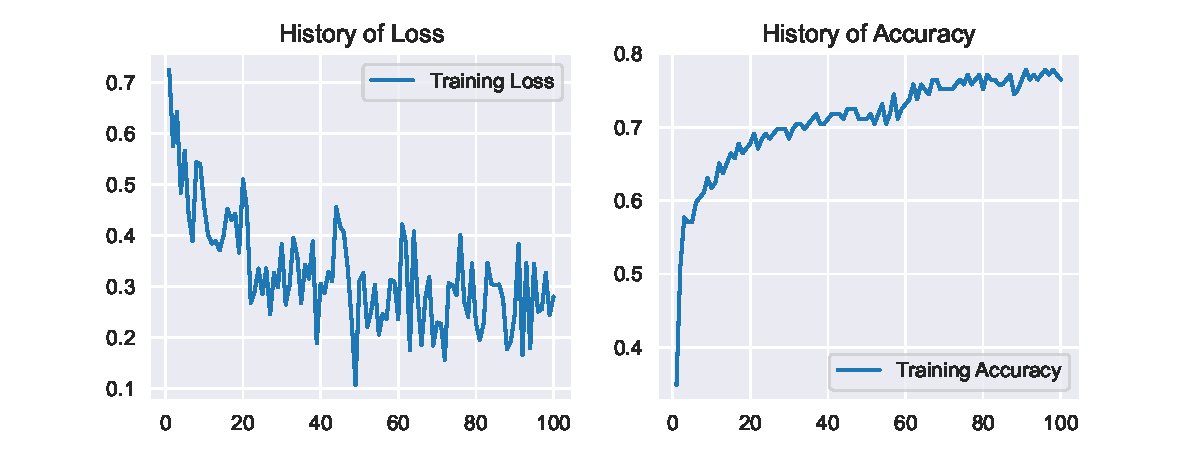
\includegraphics[scale=0.8]{figures/custom_nn_training.pdf}
\caption{Training History of Custom Neural Network Implementation}
\label{custom_nn_history}
\end{figure}

\subsubsection{Custom Neural Network Performance Evaluation}
The fitted model achieves a training accuracy of 72\% and a test accuracy of 74\% (\ref{custom_nn_evaluation}). The model is best at predicting class 1, 2 and 7 correct, which is logical since these are the majority classes. Except for the minority class 3, that is very similar to class 1 and 2 (as seen from the EDA), the model does an overall good job of classifying.

\begin{table}[!ht]
\begin{subtable}[c]{0.4\textwidth}
\footnotesize
\centering
\begin{tabular}{ c | c }
 \toprule
 Evaluation Metric & Score  \\
 \midrule 
 Training Accuracy & 72\% \\
 Test Accuracy & 74\% \\
 \bottomrule
\end{tabular}
\captionsetup{justification=centering,margin=1cm}
\subcaption{Custom Neural Network Accuracy Scores on Training and Test Split}
\end{subtable}
\begin{subtable}[c]{0.6\textwidth}
\footnotesize
\centering
\begin{tabular}{c | c c c r}
Class & Precision & Recall & F-Score & Support\\
\midrule
1   &    0.70  &    0.90  &    0.79   &     21 \\
2   &    0.73  &    0.70  &    0.71   &     23 \\
3   &    0.00  &    0.00  &    0.00   &      5 \\
5   &    0.60  &    0.75  &    0.67   &      4 \\
6   &    0.67  &    0.67  &    0.67   &      3 \\
7   &    1.00  &    0.89  &    0.94   &      9 \\
\midrule
    accuracy  &          &         &   0.74  &  65 \\
   macro avg  &   0.62   &   0.65  &   0.63  &  65 \\
weighted avg  &   0.69   &   0.74  &   0.71  &  65 \\ 
\end{tabular}
\captionsetup{justification=centering,margin=1cm}
\subcaption{Custom Neural Network Classification Report on Test Split}
\end{subtable}
\caption{Custom Neural Network Performance Evaluation}
\label{custom_nn_evaluation}
\end{table}



% ---------------------------- KERAS --------------
\textbf{Keras Implementation. }
Similarly, the neural network architecture for the Keras neural network was mostly derived through trial-and-error. A final configuration of a simple, neural network with a single hidden, ReLu-activated layer of 50 neurons, with an \class{Adam()} optimiser set to a learning rate of $0.005$ and optimising for cross-entropy loss on the entire batch (batch gradient descent) for each epoch was found to give good results. 
Using the \class{EarlyStopping()} callback, the training process was monitored, such that a continuous increase of the validation loss over $2$ epochs would stop the fitting of the model. This prevented overfitting. 
\newline

\begin{comment}
\begin{lstlisting}[language=Python, caption=Keras Neural Network Setup]
    # neural network architecture
    nn = Sequential()
    nn.add(Dense(50, input_dim=9, activation='relu', name='fc1'))
    nn.add(Dense(6, activation='softmax', name='output'))

    # define optimiser, loss and optimisation target
    nn.compile(optimizer=Adam(lr=0.005),
               loss='categorical_crossentropy', 
               metrics=['accuracy'])
            
    # early stopping
    es = EarlyStopping(monitor='val_loss', patience=2, verbose=1)
    
    # fitting neural network
    history = nn.fit(X_train, y_train_hot,
                     batch_size=len(X_train), # batch gradient descent
                     epochs=epochs,
                     verbose=2,
                     validation_split=0.2,
                     callbacks=[es]) # train with validation split (here test data)
\end{lstlisting}
\end{comment}

With this configuration, the model callback was reached after $\sim 80$ epochs. The training history is depicted in Figure \ref{keras_nn_history} and reveals that the loss continuously decreased for the training split, and was stopped just as the validation loss was beginning to increase again. 

\begin{figure}[ht]
\centering
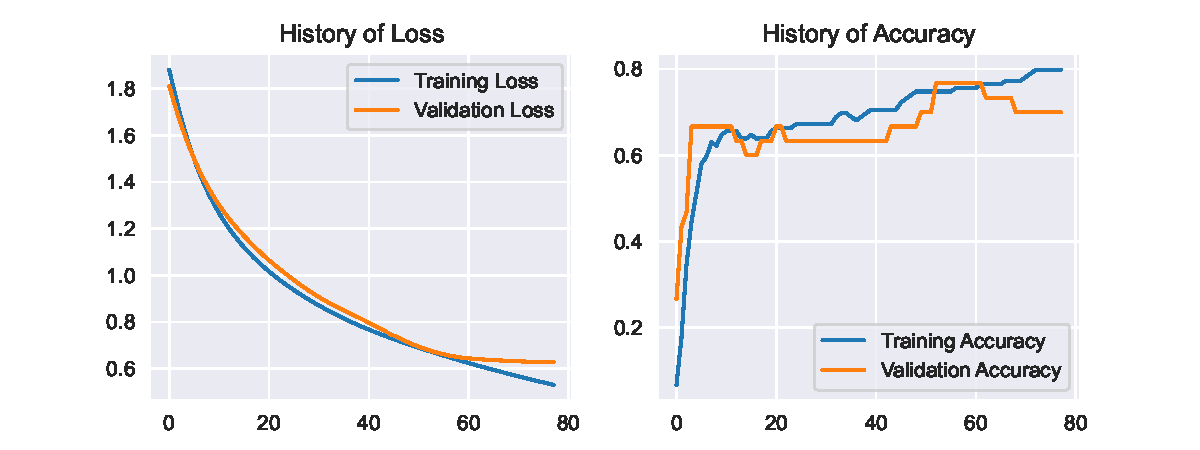
\includegraphics[scale=0.8 ]{figures/keras_nn_training.pdf}
\caption{Training History of Keras Neural Network Implementation}
\label{keras_nn_history}
\end{figure}

\subsubsection{Keras Neural Network Performance Evaluation}
As can be seen from the history of accuracies, the final trained neural network achieves a training and validation accuracy of roughly 80\%.  The validation score for this model is a good estimate for the test accuracy, which is 75\% (Figure \ref{keras_nn_evaluation}). From the classification report (Figure \ref{keras_nn_evaluation}) it becomes clear, that the model does well on the better separated classes 6 and 7. It has more difficulty separating the closely related classes 1, 2 and 3 and, in fact, never predicts the minority class 3. Nevertheless, the overall classification result is good.
\newline

\begin{table}[!ht]
\begin{subtable}[c]{0.4\textwidth}
\footnotesize
\centering
\begin{tabular}{ c | c }
 \toprule
 Evaluation Metric & Score  \\
 \midrule 
 Training Accuracy & 78\% \\
 Test Accuracy & 75\% \\
 \bottomrule
\end{tabular}
\captionsetup{justification=centering,margin=1cm}
\subcaption{Keras Neural Network Accuracy Scores on Training and Test Split}
\end{subtable}
\begin{subtable}[c]{0.6\textwidth}
\footnotesize
\centering
\begin{tabular}{c | c c c r}
Class & Precision & Recall & F-Score & Support\\
\midrule
1   &    0.72   &   0.86  &    0.78  &      21 \\
2   &    0.77   &   0.74  &    0.76  &      23 \\
3   &    0.00   &   0.00  &    0.00  &       5 \\
5   &    0.75   &   0.75  &    0.75  &       4 \\
6   &    0.75   &   1.00  &    0.86  &       3 \\
7   &    1.00   &   0.89  &    0.94  &       9 \\
\midrule
    accuracy   &           &         &    0.75   &     65 \\
   macro avg   &    0.67   &   0.71  &    0.68   &     65 \\
weighted avg   &    0.73   &   0.75  &    0.74   &     65 \\
\end{tabular}
\captionsetup{justification=centering,margin=1cm}
\subcaption{Keras Neural Network Classification Report on Test Split}
\end{subtable}
\caption{Keras Neural Network Performance Evaluation}
\label{keras_nn_evaluation}
\end{table}

\subsection{Random Forest}
\subsubsection{Introduction}
The statistical observation of the wisdom-of-the-crowd motivated the emergence of so-called ensemble methods in the cosmos of machine learning. Ensemble methods are groups of predictors, that collectively construct the ensemble's decision \cite{introStats}. 

One of the most popular ensemble-methods is the so-called \class{RandomForestClassifier()}. It refers to a series of individual decision trees  independently trained on random sub-samples and randomly selected sets of features of the input data to generate non-correlated classifiers. The final-decision is then attributed to the class being predicted by the largest number of individual trees (hard voting-classifier) \cite{introStats}.

\subsubsection{Random Forest Model Selection}
The model-selection-pipeline for the \class{RandomForestClassifier()} was similar to that of the single decision tree. Again, a pipeline that involved scaling the features was used, and grid searched for a set of hyper parameters in order to find the configuration of hyper parameters that best generalise. Within training, the hyper parameters \code{n_estimators}, \code{criterion}, \code{bootstrap} (sampling from original data with or without replacement) and \code{max_depth} were searched.
\newline 

\begin{comment}
\begin{lstlisting}[language=Python, caption=RandomForestClassifier Pipeline and GridSearch Setup]
    # define pipeline
    pipe = Pipeline(steps=[('scaler', scaler),
                           ('random_forest', RandomForestClassifier(random_state=1))])

    # define hyper parameters to grid search
    params = {'random_forest__n_estimators': [20, 50, 100],
              'random_forest__max_depth': list(range(5, 10)) + [None],
              'random_forest__bootstrap': [False, True],
              'random_forest__criterion': ['entropy', 'gini']
             }
\end{lstlisting}
\end{comment}

\subsubsection{Random Forest Performance Evaluation}
The grid search returned that the best-generalising random forest classifier uses 100 predictors, Gini-impurity as a loss-function, bootstrapped random sub-samples of the training data and trains each tree to a maximal depth of 8. This fitted model has a training accuracy of 100\%, while still having a high mean validation accuracy of 77\% encountered during the 5-fold cross validation. The accuracy on the final test set is 83\%. 

\begin{table}[!ht]
\begin{subtable}[c]{0.4\textwidth}
\footnotesize
\centering
\begin{tabular}{ c | c }
 \toprule
 Evaluation Metric & Score  \\
 \midrule 
 Training Accuracy & 100\% \\
 Validation Accuracy & 77\% \\
 Test Accuracy & 83\% \\
 \bottomrule
\end{tabular}
\captionsetup{justification=centering,margin=1cm}
\subcaption{Random Forest Accuracy Scores on Training, Validation and Test Split}
\end{subtable}
\begin{subtable}[c]{0.6\textwidth}
\footnotesize
\centering
\begin{tabular}{c | c c c r}
Class & Precision & Recall & F-Score & Support\\
\midrule
1   &  0.95  &  0.95  &  0.95  &  21\\ 
2   &  0.83  &  0.83  &  0.83  &  23\\
3   &  0.00  &  0.00  &  0.00  &   5\\
5   &  0.50  &  1.00  &  0.67  &   4\\
6   &  0.75  &  1.00  &  0.86  &   3\\
7   &  1.00  &  0.89  &  0.94  &   9\\
\midrule
    accuracy  &        &        &  0.83  &  65\\
   macro avg  &  0.67  &  0.78  &  0.71  &  65\\
weighted avg  &  0.80  &  0.83  &  0.81  &  65\\
\end{tabular}
\captionsetup{justification=centering,margin=1cm}
\subcaption{Random Forest Classification Report on Test Split}
\end{subtable}
\caption{Random Forest Performance Evaluation}
\label{random_forest_evaluation}
\end{table}

